\documentclass[12pt]{extarticle}

\usepackage{fancyhdr}
\pagestyle{fancy}
\fancyhead[R]{HW \#\thehwnumber}
\fancyhead[C]{\textbf{Math 130B}}
\fancyhead[L]{Eli Griffiths}


\usepackage{fancyhdr}
\pagestyle{fancy}
\fancyhead[R]{\textbf{CS 164: Homework \#2}}
\fancyhead[L]{Eli Griffiths}

\usepackage{algorithm}
\usepackage{algpseudocode}
\usepackage{physics}

\usepackage{tikz}
\usetikzlibrary{arrows.meta}

\newtcolorbox{solution}{
	breakable,
	coltitle = black,
	colback = white,
	frame hidden,
	boxrule = 0pt,
	boxsep = 0pt,
	borderline west={2pt}{0pt}{black},
	sharp corners = all,
	enhanced,
}

\begin{document}

\section*{Problem 1}
Let $S$ be a set of $n$ disjoint line segments whose upper endpoints lie on the line $y = 1$ and whose lower endpoints lie on the line $y = 0$. These segments partition the horizontal strip $[-\infty, \infty] \times [0,1]$ into $n+1$ regions. Give an $O(n \log n)$ time algorithm to build a binary search tree on the segments in $S$ such that the region containing a query point can be determined in $O(\log n)$ time. Also describe the query algorithm in detail.

\begin{solution}
    The algorithm for building the binary search tree over $S$ and querying it is fairly simple. The idea is that since the segments are disjoint, a binary search tree can be used to reprsent when segments are to left and right of each other based purely on the $x$-coordinate of their upper endpoint. Then when querying a point $p$, it boils down to traversing the tree left or right based on if the point is oriented left or right of the current segment, and then returning the two correct neighboring segments when a leaf node is reached.

    \begin{algorithm}[H]
        \caption{\textsc{CreatePartitionTree}($S$)}
        \begin{enumerate}
            \item Create empty AVL tree
            \item For every segment, insert it into the tree based on the $x$-coordinate of its upper endpoint
            \item Return the tree
        \end{enumerate}
    \end{algorithm}

    \begin{algorithm}[H]
        \caption{\textsc{QueryPartitionTree}($\mathcal{T}, p$)}
        \begin{enumerate}
            \item Start at the root node/segment $s$ of $\mathcal{T}$
            \item While $s$ is not a leaf node
            \begin{itemize}
                \item Check if $p$ is to the left or right of $s$ and update $s$ to be the corresponding left or right node
            \end{itemize}
            \item If $p$ is now to the left of $s$, then return the current segment and the previous segment in the tree
            \item If $p$ is now to the right of $s$, then return the current segment and the next segment in the tree
        \end{enumerate}
    \end{algorithm}

    Breaking down the running times of each routine:
    \begin{enumerate}[leftmargin=5cm]
        \item[\textsc{CreatePartitionTree})]
            Iterating over every line segment takes $O(n)$ time, and for each segment we are inserting it into an AVL tree which takes $O(\log n)$ time. Therefore in total creating the partition tree takes $O(n \log n)$ time.
        \item[\textsc{QueryPartitionTree})]
            Traversing the search tree takes only $O(\log n)$ time. Finding the previous or next node in the tree can also be done in $O(\log n)$ time. Therefore in total querying takes $O(\log n)$ time.
    \end{enumerate}
    Both algorithms therefore satisfy the time complexity requirements.
\end{solution}

\section*{Problem 2}

The intersection detection problem for a set $S$ of n line segments is to determine whether there exists a pair of segments in $S$ that intersect. Give a plane sweep algorithm that solves the intersection detection problem in $O(n \log n)$ time.

\begin{solution}
    The plane sweep algorithm outlined in the textbook can be used with the modification that when any intersection is encountered, it returns early. The plane sweep algorithm has a time complexity of $O((n+k)\log n)$ where $k$ is the number of detected intersections, but the early return restricts $k$ to be either $0$ or $1$. Therefore $k$ is bounded independent of $n$ meaning the time complexity of this modified plane sweep is $O((n+1) \log n) = O(n \log n)$.
\end{solution}

\section*{Problem 3}
Give an example of a doubly-connected edge list where for an edge $e$ the faces 

$\textsc{IncidentFace}(\vec{e})$ and $\textsc{IncidentFace}(\textsc{Twin}(\vec{e}))$ are the same.

\begin{solution}
    An example that satisfies this condition is a DCEL where there are two vertices and a single edge going between them. Then there is simply one face with both half deges inside it, meaning both will have the same incident face and both half edges are twins.
    \begin{figure}[H]
        \centering
        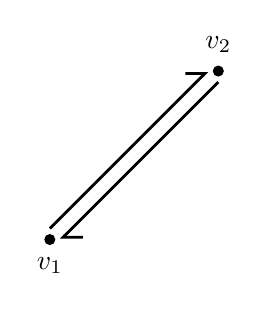
\begin{tikzpicture}[
            edge/.style = {
                line width=1pt,
                -{Straight Barb[left,length=5pt]}
            }
            ]
            % Nodes
            \node (v1) at (-1,-1) {};
            \node (v2) at ( 1, 1) {};

            \newcommand{\sep}{0.07}

            \fill (v1) ++(-\sep, -\sep) circle (2pt) node[below=3pt] {$v_1$};
            \fill (v2) ++( \sep,  \sep) circle (2pt) node[above=3pt] {$v_2$};
            \draw[edge] (v1) ++(-\sep,  \sep) -- +( 2,  2);
            \draw[edge] (v2) ++( \sep, -\sep) -- +(-2, -2);
        \end{tikzpicture}
        \caption{Illustration of example DCEL configuration}
    \end{figure}
\end{solution}

\section*{Problem 4}
Given a doubly-connected edge list representation of a subdivision where $\textsc{Twin}(\vec{e}) = \textsc{Next}(\vec{e})$ holds for every half-edge $e$, how many faces can the subdivision have at most?

\begin{solution}
    Assume that we have a DCEL satisfting the given property. Then we know
    \[
        \textsc{IncidentFace}(\textsc{Twin}(\vec{e})) = 
        \textsc{IncidentFace}(\textsc{Next}(\vec{e})) 
    .\]
    But we also know that $ \textsc{IncidentFace}(\textsc{Next}(\vec{e})) = \textsc{IncidentFace}(\vec{e})$. Therefore
    \[
        \textsc{IncidentFace}(\vec{e}) = 
        \textsc{IncidentFace}(\textsc{Twin}(\vec{e})) 
    \]
    which holds for every half edge $e$. But this means that there is no edge that is on the boundary of two faces, otherwise there would be a half-edge pair where the incident faces between them are different. Therefore there is at most $1$ face in this setup.
\end{solution}

\section*{Problem 5}
Suppose that a doubly-connected edge list of a connected subdivision is given. Give pseudocode for an algorithm that lists all faces with vertices that appear on the outer boundary.

\begin{solution}
    The idea behind this algorithm is that we first find an edge that is guaranteed to be on the outer boundary. Then we can use that edge to walk around the boundary, keeping track of the inner faces that have an edge adjacent to the origin of the current edge. Finding this edge is simple as we can just find which face has no outer component and then use its inner component as the edge on the boundary. This algorithm only requires the list of faces from the DCEL. In total,
    \begin{algorithm}[H]
        \caption{\textsc{FindBoundaryFaces}($\mathcal{F}$)}
        \begin{algorithmic}[1]
            \newcommand{\curr}{e_\text{curr}}

            \State $\mathrm{F} \gets$ Empty face list
            \State $f \gets $ Face in $\mathcal{F}$ with $nil$ outer component
            \State $e_0 \gets$ \Call{InnerComponent}{$f$}
            \State $\curr \gets e_0$ 

            \State Append \Call{IncidentFace}{$\curr$} to $\mathrm{F}$

            \Repeat \Comment{Loop over all outer edges}
                \State $e_v \gets $ \textsc{Next}(\textsc{Twin}($\curr$))
                \Repeat \Comment{Loop over all edges originating from $\curr$}
                    \State Append \Call{IncidentFace}{$e_v$} to $\mathrm{F}$
                    \State $e_v \gets $ \textsc{Next}(\textsc{Twin}($\curr$))
                \Until{$e_v = \curr$}
            \Until{$\curr = e_0$}
            \State \Return $\mathrm{F}$
        \end{algorithmic}
    \end{algorithm}
\end{solution}

\end{document}
